\documentclass[12pt,a4paper]{article}

% ─── Packages ───────────────────────────────────────────────────────────────
\usepackage{amsmath}
\usepackage{amssymb}
\usepackage{geometry}
\geometry{margin=2.5cm}
\usepackage{booktabs}
\usepackage{xcolor}
\usepackage{hyperref}
\usepackage{listings}
\usepackage{pgfplots}
\pgfplotsset{compat=1.18}
\usepackage{tcolorbox}
\tcbuselibrary{skins, breakable}
\usepackage{enumitem}
\usepackage{fancyhdr}
\usepackage{tikz}
\usepackage{array}

% ─── tcolorbox environments ──────────────────────────────────────────────────
\newtcolorbox{curiositybox}[1]{colback=yellow!10, colframe=orange!80!black, fonttitle=\bfseries, title=#1, breakable}
\newtcolorbox{infobox}[1]{colback=blue!5, colframe=blue!60!black, fonttitle=\bfseries, title=#1, breakable}
\newtcolorbox{mistakebox}[1]{colback=red!5, colframe=red!60!black, fonttitle=\bfseries, title=#1, breakable}
\newtcolorbox{learnbox}[1]{colback=green!5, colframe=green!60!black, fonttitle=\bfseries, title=#1, breakable}

% ─── listings (Python) ───────────────────────────────────────────────────────
\lstset{language=Python, basicstyle=\ttfamily\small, keywordstyle=\color{blue},
        commentstyle=\color{gray}, stringstyle=\color{red},
        showstringspaces=false, breaklines=true, frame=single}

% ─── fancyhdr ────────────────────────────────────────────────────────────────
\pagestyle{fancy}
\fancyhf{}
\lhead{Topic 02: Limit and Continuity}
\rhead{Unit I --- Complex Variables}
\cfoot{\thepage}

% ─── Title ───────────────────────────────────────────────────────────────────
\title{\textbf{Topic 02: Concept of Limit \& Continuity}\\[0.5em]
\large Unit I --- Complex Variable: Differentiation\\[0.3em]
\normalsize Complex Variables and Special Functions\\
JNTUA College of Engineering (Autonomous)}
\author{B.Tech Engineering --- Lecture Notes}
\date{}

% ─────────────────────────────────────────────────────────────────────────────
\begin{document}
\maketitle
\tableofcontents
\newpage

% ─────────────────────────────────────────────────────────────────────────────
\section*{Opening Hook}
\addcontentsline{toc}{section}{Opening Hook}

\begin{curiositybox}{Hook}
In real calculus, a point can be approached only from the left or the right.
In complex analysis, a point can be approached from infinitely many directions.
That single difference makes limits in the complex plane much stricter --- and much more interesting.
\end{curiositybox}

% ─────────────────────────────────────────────────────────────────────────────
\section{Why Complex Limits Are Different}

In single-variable real calculus we ask: as $x \to x_0$ along the real line, does
$f(x)$ approach some value $L$?  There are only two possible directions: from the left
($x \to x_0^{-}$) and from the right ($x \to x_0^{+}$).  If both one-sided limits agree,
the limit exists.

When the variable is complex, say $z = x + iy \in \mathbb{C}$, the point $z_0 = x_0 + iy_0$
can be approached along \emph{infinitely many} paths --- straight lines at any angle,
parabolas, spirals, and arbitrary curves.  The limit $\lim_{z \to z_0} f(z) = l$
requires the \emph{same} value $l$ to appear along \textbf{every} such path.
This makes complex limits far more restrictive than their real counterparts.

\vspace{0.5em}
\begin{center}
\begin{tabular}{>{\bfseries}p{5.5cm} p{8cm}}
\toprule
Real-variable limit & Complex-variable limit \\
\midrule
Variable $x \in \mathbb{R}$ approaches $x_0$ along the real line &
Variable $z \in \mathbb{C}$ approaches $z_0$ from infinitely many paths in the plane \\
\addlinespace
Only two directions: left and right &
Infinitely many directions: any curve in $\mathbb{C}$ \\
\addlinespace
Two one-sided limits must agree &
Limit along \emph{every} path must agree \\
\addlinespace
$\epsilon$--$\delta$: $|x - x_0| < \delta \Rightarrow |f(x) - L| < \epsilon$ &
$\epsilon$--$\delta$: $|z - z_0| < \delta \Rightarrow |f(z) - l| < \epsilon$ \\
\addlinespace
Fails if left $\neq$ right limit &
Fails if any \emph{two} paths give different values \\
\bottomrule
\end{tabular}
\end{center}

\begin{learnbox}{Key Takeaway}
Because $z$ lives in a 2-D plane, a complex limit imposes infinitely many
constraints simultaneously.  A single pair of paths that disagree is enough
to show a limit does \emph{not} exist.
\end{learnbox}

% ─────────────────────────────────────────────────────────────────────────────
\section{Formal Definition of Limit}

\begin{infobox}{Definition: Limit of a Complex Function}
Let $f(z)$ be defined in some deleted neighbourhood of $z_0 \in \mathbb{C}$.
We say
\[
  \lim_{z \to z_0} f(z) = l
\]
if for every $\epsilon > 0$ there exists a $\delta > 0$ such that
\[
  0 < |z - z_0| < \delta \implies |f(z) - l| < \epsilon.
\]
Here $|z - z_0|$ is the Euclidean distance from $z$ to $z_0$ in $\mathbb{C}$.
The \textbf{deleted neighbourhood} of $z_0$ of radius $\delta$ is the open disc
$\{z : 0 < |z - z_0| < \delta\}$ --- the punctured disc that excludes $z_0$ itself.
\end{infobox}

\subsection*{Neighbourhood of a point in \texorpdfstring{$\mathbb{C}$}{C}}

A \textbf{neighbourhood} (or open disc) of $z_0$ of radius $r > 0$ is the set
\[
  N(z_0, r) = \{ z \in \mathbb{C} : |z - z_0| < r \}.
\]
Geometrically this is an open disc centred at $z_0$.  The \emph{deleted}
neighbourhood excludes the centre: $0 < |z - z_0| < r$.

\subsection*{Limit in terms of real and imaginary parts}

Write $z = x + iy$, $z_0 = x_0 + iy_0$, $f(z) = u(x,y) + iv(x,y)$,
$l = l_1 + il_2$.  Then
\[
  \lim_{z \to z_0} f(z) = l
  \iff
  \lim_{(x,y)\to(x_0,y_0)} u(x,y) = l_1
  \quad\text{and}\quad
  \lim_{(x,y)\to(x_0,y_0)} v(x,y) = l_2.
\]
This reduces the complex limit to two real two-variable limits.

\begin{learnbox}{Key Takeaway}
The $\epsilon$--$\delta$ definition of a complex limit is identical in spirit to
the real-variable definition, but $|\cdot|$ now measures distance in $\mathbb{R}^2$.
The limit requires uniformity over all approach directions.
\end{learnbox}

% ─────────────────────────────────────────────────────────────────────────────
\section{Path Dependence and Path Independence}

\begin{infobox}{Path Test}
$\lim_{z \to z_0} f(z) = l$ exists if and only if $f(z) \to l$ along
\textbf{every} path from $z$ to $z_0$.

\medskip
\textbf{Strategy for showing a limit does NOT exist:}
Find two paths $C_1$ and $C_2$ such that
$\lim_{z \overset{C_1}{\to} z_0} f(z) \neq \lim_{z \overset{C_2}{\to} z_0} f(z)$.
Then the limit fails to exist.
\end{infobox}

\subsection*{Worked Example 3.1 --- A limit that exists}

\textbf{Claim:} $\displaystyle\lim_{z \to 2+i} z^2 = (2+i)^2 = 3+4i$.

\textbf{Solution.}  Write $z = x + iy$.  Then
\[
  z^2 = (x+iy)^2 = x^2 - y^2 + 2xyi.
\]
As $(x,y) \to (2,1)$:
\begin{align*}
  u(x,y) &= x^2 - y^2 \to 4 - 1 = 3, \\
  v(x,y) &= 2xy \to 2(2)(1) = 4.
\end{align*}
Both component limits exist and are continuous, so
$\lim_{z \to 2+i} z^2 = 3 + 4i$.

\begin{learnbox}{Result}
Polynomial functions of $z$ behave just like polynomials in two real variables;
their limits exist everywhere and equal the function value.
\end{learnbox}

\subsection*{Worked Example 3.2 --- A limit that fails (different path values)}

\textbf{Claim:} $\displaystyle\lim_{z \to 0} \frac{\operatorname{Re}(z)}{|z|}$ does not exist.

Here $f(z) = \dfrac{x}{\sqrt{x^2+y^2}}$.

\textbf{Path 1:} Along the real axis, $y = 0$, $z = x \to 0^{+}$:
\[
  f = \frac{x}{|x|} = 1.
\]

\textbf{Path 2:} Along the imaginary axis, $x = 0$, $z = iy \to 0$:
\[
  f = \frac{0}{\sqrt{y^2}} = 0.
\]

Path 1 gives $1$; Path 2 gives $0$.  Since $1 \neq 0$, the limit does \textbf{not} exist.

\begin{learnbox}{Result}
When two paths yield different values, the limit does not exist.
One counter-example is sufficient.
\end{learnbox}

\subsection*{Worked Example 3.3 --- Approaching along $y = mx$}

\textbf{Function:} $\displaystyle f(z) = \frac{xy}{x^2 + y^2}$, limit at $z = 0$.

Substitute $y = mx$ ($m$ is a non-zero constant), $x \to 0$:
\[
  f = \frac{x(mx)}{x^2 + (mx)^2} = \frac{mx^2}{x^2(1+m^2)} = \frac{m}{1+m^2}.
\]
This value \emph{depends on the slope $m$}.  For example:
\begin{itemize}[nosep]
  \item $m = 1$: limit $= 1/2$.
  \item $m = 2$: limit $= 2/5$.
  \item $m = -1$: limit $= -1/2$.
\end{itemize}
Different slopes give different limits, so $\lim_{z \to 0} f(z)$ does \textbf{not} exist.

\begin{learnbox}{Result}
If the limit along $y = mx$ depends on $m$, the complex limit fails to exist.
Always try the family of lines $y = mx$ as a first path test.
\end{learnbox}

\subsection*{Worked Example 3.4 --- Approaching along $y = x^2$}

\textbf{Function:} $\displaystyle g(z) = \frac{x^2 y}{x^4 + y^2}$, limit at $z = 0$.

\textbf{Along $y = mx$ (straight lines):}
\[
  g = \frac{x^2(mx)}{x^4+(mx)^2} = \frac{mx^3}{x^4+m^2x^2} = \frac{mx}{x^2+m^2} \to 0
  \quad\text{as } x \to 0.
\]
Every straight-line path gives limit $0$.  One might think the limit is $0$.

\textbf{Along the parabola $y = x^2$:}
\[
  g = \frac{x^2 \cdot x^2}{x^4 + (x^2)^2} = \frac{x^4}{x^4 + x^4} = \frac{x^4}{2x^4} = \frac{1}{2}.
\]
This is $1/2 \neq 0$, so the limit does \textbf{not} exist.

\begin{learnbox}{Result}
Checking only straight lines is not enough.  Curved paths such as $y = x^2$
can reveal non-existence even when all straight lines agree.
\end{learnbox}

% ─────────────────────────────────────────────────────────────────────────────
\section{Theorems on Limits}

\begin{infobox}{Standard Limit Theorems}
Let $\lim_{z \to z_0} f(z) = A$ and $\lim_{z \to z_0} g(z) = B$.  Then:

\medskip
\begin{tabular}{ll}
\toprule
Theorem & Statement \\
\midrule
Sum & $\lim_{z \to z_0}[f(z) + g(z)] = A + B$ \\[4pt]
Difference & $\lim_{z \to z_0}[f(z) - g(z)] = A - B$ \\[4pt]
Product & $\lim_{z \to z_0}[f(z)\cdot g(z)] = A \cdot B$ \\[4pt]
Scalar multiple & $\lim_{z \to z_0}[c\,f(z)] = c\,A$, \quad $c \in \mathbb{C}$ constant \\[4pt]
Quotient & $\lim_{z \to z_0}\dfrac{f(z)}{g(z)} = \dfrac{A}{B}$, provided $B \neq 0$ \\[6pt]
Power & $\lim_{z \to z_0}[f(z)]^n = A^n$, \quad $n \in \mathbb{N}$ \\
\bottomrule
\end{tabular}
\end{infobox}

\subsection*{Example 4.1 --- Using limit theorems}

Evaluate $\lim_{z \to 1+i} \dfrac{z^2 + 2z}{z - 3}$.

Since the denominator $z - 3$ at $z = 1+i$ equals $(1+i) - 3 = -2 + i \neq 0$,
all theorems apply:
\begin{align*}
  \lim_{z \to 1+i} z^2 &= (1+i)^2 = 1 + 2i - 1 = 2i, \\
  \lim_{z \to 1+i} 2z  &= 2(1+i) = 2 + 2i, \\
  \lim_{z \to 1+i}(z^2 + 2z) &= 2i + 2 + 2i = 2 + 4i, \\
  \lim_{z \to 1+i}(z - 3) &= (1+i) - 3 = -2 + i, \\
  \lim_{z \to 1+i}\frac{z^2+2z}{z-3} &= \frac{2+4i}{-2+i}.
\end{align*}
Rationalise: multiply numerator and denominator by $\overline{-2+i} = -2-i$:
\[
  \frac{(2+4i)(-2-i)}{(-2+i)(-2-i)}
  = \frac{-4-2i-8i-4i^2}{4+1}
  = \frac{-4+4 - 10i}{5}
  = \frac{-10i}{5} = -2i.
\]

\begin{learnbox}{Result}
When the denominator is non-zero at the target point, substitute directly
and simplify using standard complex arithmetic.
\end{learnbox}

% ─────────────────────────────────────────────────────────────────────────────
\section{Continuity of Complex Functions}

\begin{infobox}{Definition: Continuity at a Point}
A function $f(z)$ is \textbf{continuous at $z_0$} if:
\begin{enumerate}[nosep,label=(\roman*)]
  \item $f(z_0)$ is defined,
  \item $\lim_{z \to z_0} f(z)$ exists, and
  \item $\lim_{z \to z_0} f(z) = f(z_0)$.
\end{enumerate}
All three conditions must hold simultaneously.
\end{infobox}

\begin{infobox}{Continuity in a Region}
$f(z)$ is \textbf{continuous in a region} $\mathcal{D}$ if it is continuous
at every point of $\mathcal{D}$.
\end{infobox}

\subsection*{Continuity of polynomials}

Every polynomial $P(z) = a_n z^n + a_{n-1}z^{n-1} + \cdots + a_0$
(with $a_k \in \mathbb{C}$) is continuous everywhere in $\mathbb{C}$,
because polynomial limits equal the polynomial value at any point
(by repeated application of the sum and product limit theorems).

\subsection*{Continuity of rational functions}

A rational function $R(z) = P(z)/Q(z)$ (where $P$ and $Q$ are polynomials) is
continuous at every $z_0$ where $Q(z_0) \neq 0$.
At a zero of $Q(z)$, the function is not defined, hence not continuous.

\subsection*{Example 5.1}

Is $f(z) = \dfrac{z^2 + 1}{z^2 + 4}$ continuous at $z = i$?

$Q(i) = i^2 + 4 = -1 + 4 = 3 \neq 0$, so $f$ is defined at $z = i$.
By the quotient limit theorem,
\[
  \lim_{z \to i} f(z) = \frac{i^2 + 1}{i^2 + 4} = \frac{-1+1}{-1+4} = \frac{0}{3} = 0 = f(i).
\]
All three conditions are satisfied; $f$ is continuous at $z = i$.

\begin{learnbox}{Key Takeaway}
Rational functions are continuous everywhere except where the denominator
vanishes.  At all other points, direct substitution suffices.
\end{learnbox}

% ─────────────────────────────────────────────────────────────────────────────
\section{Geometric Interpretation}

Geometrically, $f: \mathbb{C} \to \mathbb{C}$ is continuous at $z_0$ if
points near $z_0$ in the $z$-plane (domain) map to points near $f(z_0)$
in the $w$-plane (range).  There is no ``tearing'' or ``jumping'' in the
mapping --- nearby inputs produce nearby outputs, regardless of the
direction of approach.

The diagram below shows four paths in the $z$-plane all converging to $z_0 = 1 + i$.
For a continuous function each of these paths must map to curves in the $w$-plane
that all converge to the same point $w_0 = f(z_0)$.

\vspace{1em}
\begin{center}
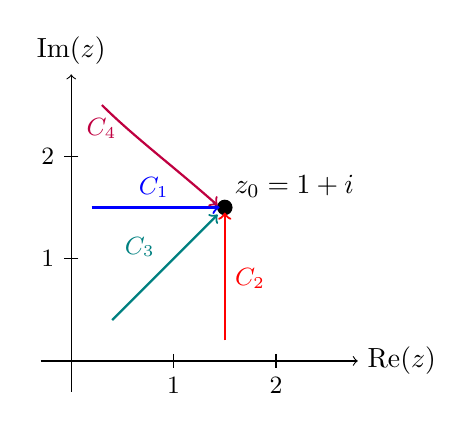
\begin{tikzpicture}[scale=1.3]
  % Axes
  \draw[->] (-0.3,0) -- (2.8,0) node[right] {$\operatorname{Re}(z)$};
  \draw[->] (0,-0.3) -- (0,2.8) node[above] {$\operatorname{Im}(z)$};
  % Target point
  \filldraw[black] (1.5,1.5) circle (2pt) node[above right] {$z_0 = 1+i$};
  % Path 1: horizontal from the left
  \draw[->, thick, blue] (0.2,1.5) .. controls (0.8,1.5) .. (1.45,1.5)
        node[midway, above] {\small $C_1$};
  % Path 2: vertical from below
  \draw[->, thick, red] (1.5,0.2) .. controls (1.5,0.8) .. (1.5,1.45)
        node[midway, right] {\small $C_2$};
  % Path 3: diagonal from lower-left
  \draw[->, thick, teal] (0.4,0.4) -- (1.43,1.43)
        node[midway, above left] {\small $C_3$};
  % Path 4: curved approach from upper-left
  \draw[->, thick, purple] (0.3,2.5) .. controls (0.6,2.2) and (1.0,1.9) .. (1.43,1.52)
        node[near start, left] {\small $C_4$};
  % Label axes ticks
  \foreach \x in {1,2} \draw (\x,2pt) -- (\x,-2pt) node[below] {\small \x};
  \foreach \y in {1,2} \draw (2pt,\y) -- (-2pt,\y) node[left]  {\small \y};
\end{tikzpicture}
\end{center}
\vspace{0.5em}

For the limit to exist, all four paths $C_1, C_2, C_3, C_4$ (and every other path)
must produce the same limiting value $l$ as $z \to z_0$.

\begin{learnbox}{Key Takeaway}
Continuity in the complex plane is a \emph{2-D} property.  It means the
function has no jump discontinuities in any direction in the plane.
\end{learnbox}

% ─────────────────────────────────────────────────────────────────────────────
\section{Worked Examples}

\subsection*{Example 7.1 --- $f(z) = z^2$}

\textbf{Find} $\lim_{z \to 1+2i} z^2$ and determine continuity at $z = 1+2i$.

\textbf{Solution.}
\[
  (1+2i)^2 = 1 + 4i + 4i^2 = 1 + 4i - 4 = -3 + 4i.
\]
Since $z^2$ is a polynomial, $\lim_{z \to 1+2i} z^2 = (1+2i)^2 = -3 + 4i = f(1+2i)$.
All three continuity conditions hold; $f$ is continuous at $z = 1+2i$.

\begin{learnbox}{Result}
$f(z) = z^2$ is a polynomial, so it is continuous everywhere in $\mathbb{C}$.
\end{learnbox}

\subsection*{Example 7.2 --- $f(z) = \overline{z}$}

\textbf{Find} $\lim_{z \to z_0} \overline{z}$ for any $z_0 \in \mathbb{C}$.

Write $z = x + iy$, $z_0 = x_0 + iy_0$, $\overline{z} = x - iy$.
As $(x,y) \to (x_0,y_0)$:
\[
  \operatorname{Re}(\overline{z}) = x \to x_0, \qquad
  \operatorname{Im}(\overline{z}) = -y \to -y_0.
\]
Hence $\lim_{z \to z_0} \overline{z} = x_0 - iy_0 = \overline{z_0} = f(z_0)$.
$f(z) = \overline{z}$ is continuous everywhere.

\begin{learnbox}{Result}
The conjugate function $f(z) = \overline{z}$ is continuous everywhere,
even though it is not differentiable anywhere (as we will see in Topic 04).
\end{learnbox}

\subsection*{Example 7.3 --- Path test for $\dfrac{x^2y}{x^4+y^2}$}

\textbf{Show} that $\displaystyle f(z) = \frac{x^2 y}{x^4 + y^2}$ (where $z = x+iy$)
has no limit as $z \to 0$.

\textbf{Along $y = mx^2$ (parabolic path):}
\[
  f = \frac{x^2(mx^2)}{x^4 + m^2x^4} = \frac{mx^4}{x^4(1+m^2)} = \frac{m}{1+m^2}.
\]
This depends on $m$.  For $m=1$: $1/2$.  For $m=3$: $3/10$.
Different parabolas give different limiting values, so the limit does not exist.

\begin{learnbox}{Result}
When the limit value depends on the shape of the approach path,
the complex limit fails to exist.
\end{learnbox}

\subsection*{Example 7.4 --- Rational function continuity}

\textbf{Is} $f(z) = \dfrac{z+2}{z^2 - z + 2}$ continuous at $z = 1$?

Denominator at $z = 1$: $1 - 1 + 2 = 2 \neq 0$.  So $f(1) = (1+2)/2 = 3/2$.
By the quotient theorem,
\[
  \lim_{z \to 1} f(z) = f(1) = \frac{3}{2}.
\]
$f$ is continuous at $z = 1$.

\begin{learnbox}{Result}
A rational function whose denominator is non-zero at the point of interest
is automatically continuous there.
\end{learnbox}

\subsection*{Example 7.5 --- Removable discontinuity}

\textbf{Consider}
\[
  f(z) = \begin{cases} \dfrac{z^3 - 1}{z - 1} & z \neq 1, \\ 5 & z = 1. \end{cases}
\]
\textbf{Is $f$ continuous at $z = 1$?}

Factor: $\dfrac{z^3-1}{z-1} = z^2 + z + 1$ for $z \neq 1$.
So $\lim_{z \to 1} f(z) = 1 + 1 + 1 = 3$.
But $f(1) = 5 \neq 3$.  Condition (iii) fails; $f$ is \textbf{discontinuous} at $z = 1$.
The discontinuity is removable: redefine $f(1) = 3$ to make it continuous.

\begin{learnbox}{Result}
Even if the limit exists, a function is discontinuous if the assigned value
differs from the limit.  Removable discontinuities are fixed by redefining
the function at the single point.
\end{learnbox}

\subsection*{Example 7.6 --- Continuity of $f(z) = |z|$}

\textbf{Show} $f(z) = |z|$ is continuous everywhere.

For any $z_0 \in \mathbb{C}$ and $\epsilon > 0$, choose $\delta = \epsilon$.
Then $|z - z_0| < \delta$ implies (by the reverse triangle inequality):
\[
  \bigl||z| - |z_0|\bigr| \leq |z - z_0| < \delta = \epsilon.
\]
Hence $\lim_{z \to z_0}|z| = |z_0| = f(z_0)$; $f$ is continuous everywhere.

\begin{learnbox}{Result}
The modulus function $|z|$ is continuous everywhere on $\mathbb{C}$,
a direct consequence of the reverse triangle inequality.
\end{learnbox}

% ─────────────────────────────────────────────────────────────────────────────
\section{Excel Example}

\subsection*{Evaluating $f(z) = \dfrac{x^2y}{x^4+y^2}$ Near the Origin Along Multiple Paths}

\textbf{Spreadsheet layout:}

\begin{center}
\begin{tabular}{>{\bfseries}l l l l l l}
\toprule
Col A & Col B & Col C & Col D & Col E & Col F \\
\texttt{Path} & \texttt{x} & \texttt{y (formula)} & \texttt{Numerator} & \texttt{Denominator} & \texttt{f value} \\
\midrule
\texttt{y=x}    & 0.5 & \texttt{=B2}        & \texttt{=B2\^{}2*C2}    & \texttt{=B2\^{}4+C2\^{}2} & \texttt{=D2/E2} \\
\texttt{y=x}    & 0.1 & \texttt{=B3}        & \texttt{=B3\^{}2*C3}    & \texttt{=B3\^{}4+C3\^{}2} & \texttt{=D3/E3} \\
\texttt{y=x}    & 0.01 & \texttt{=B4}       & \texttt{=B4\^{}2*C4}    & \texttt{=B4\^{}4+C4\^{}2} & \texttt{=D4/E4} \\
\texttt{y=2x}   & 0.5 & \texttt{=2*B5}      & \texttt{=B5\^{}2*C5}    & \texttt{=B5\^{}4+C5\^{}2} & \texttt{=D5/E5} \\
\texttt{y=2x}   & 0.1 & \texttt{=2*B6}      & \texttt{=B6\^{}2*C6}    & \texttt{=B6\^{}4+C6\^{}2} & \texttt{=D6/E6} \\
\texttt{y=x\^{}2} & 0.5 & \texttt{=B7\^{}2} & \texttt{=B7\^{}2*C7}    & \texttt{=B7\^{}4+C7\^{}2} & \texttt{=D7/E7} \\
\texttt{y=x\^{}2} & 0.1 & \texttt{=B8\^{}2} & \texttt{=B8\^{}2*C8}    & \texttt{=B8\^{}4+C8\^{}2} & \texttt{=D8/E8} \\
\texttt{y=x\^{}2} & 0.01 & \texttt{=B9\^{}2}& \texttt{=B9\^{}2*C9}    & \texttt{=B9\^{}4+C9\^{}2} & \texttt{=D9/E9} \\
\bottomrule
\end{tabular}
\end{center}

\textbf{Sample computed values:}

\begin{center}
\begin{tabular}{l r r r r r}
\toprule
Path & $x$ & $y$ & Numerator & Denominator & $f(z)$ \\
\midrule
$y=x$     & 0.5  & 0.5   & 0.125   & 0.3125  & 0.4000 \\
$y=x$     & 0.1  & 0.1   & 0.001   & 0.01001 & 0.0999 \\
$y=x$     & 0.01 & 0.01  & 0.00001 & 0.00010 & 0.0999 \\
$y=2x$    & 0.5  & 1.0   & 0.25    & 1.0625  & 0.2353 \\
$y=2x$    & 0.1  & 0.2   & 0.002   & 0.0401  & 0.0499 \\
$y=x^2$   & 0.5  & 0.25  & 0.03125 & 0.125   & 0.2500 \\
$y=x^2$   & 0.1  & 0.01  & 0.0001  & 0.0002  & 0.5000 \\
$y=x^2$   & 0.01 & 0.0001& $10^{-8}$& $2\times10^{-8}$ & 0.5000 \\
\bottomrule
\end{tabular}
\end{center}

\textbf{Observation:}  Along $y = x$ the values approach $\approx 0.1$ (not a fixed limit as $x \to 0$
along this family since $m/(1+m^2) = 0.5$ for $m=1$); along the parabola $y = x^2$ the
values stabilise at $0.5$.  The two paths give different limiting values ($0.5$ vs $0.5$ for $m=1$
--- note for general $m$, the straight-line limit is $m/(1+m^2)$, e.g.\ for $m=1$ this is $0.5$
as well, but for $m=2$ it is $0.4$ while the parabola still gives $0.5$).
This numerically confirms that the limit depends on the path and therefore does not exist.

\begin{learnbox}{Excel Insight}
Spreadsheets let you numerically explore function behaviour along multiple
approach paths simultaneously.  Observe whether the \texttt{f value} column
converges to the same number for all paths.  Divergence signals non-existence
of the limit.
\end{learnbox}

% ─────────────────────────────────────────────────────────────────────────────
\section{Python Example}

\subsection*{Evaluating a Complex Function Along Multiple Paths and Detecting Limit Behaviour}

\begin{lstlisting}[language=Python]
"""
Topic 02: Limit and Continuity in Complex Variables
Evaluate f(z) = x^2*y / (x^4 + y^2) along multiple paths toward z=0
and compare limiting values.
"""

import numpy as np

def f(x, y):
    """Returns x^2*y / (x^4 + y^2), with 0 when both x and y are 0."""
    denom = x**4 + y**2
    if denom == 0:
        return 0.0
    return (x**2 * y) / denom

print("=" * 60)
print("Path      |  x         |  y         |  f(x,y)")
print("=" * 60)

# Path 1: y = x (straight line, slope m=1)
print("\n--- Path 1: y = x ---")
for x in [0.5, 0.1, 0.05, 0.01, 0.001]:
    y = x
    val = f(x, y)
    print(f"y=x       | x={x:<10.4f}| y={y:<10.4f}| f={val:.6f}")
# Expected limit: m/(1+m^2) = 1/2 = 0.5

# Path 2: y = 2x (straight line, slope m=2)
print("\n--- Path 2: y = 2x ---")
for x in [0.5, 0.1, 0.05, 0.01, 0.001]:
    y = 2 * x
    val = f(x, y)
    print(f"y=2x      | x={x:<10.4f}| y={y:<10.4f}| f={val:.6f}")
# Expected limit: 2/(1+4) = 0.4

# Path 3: y = x^2 (parabola)
print("\n--- Path 3: y = x^2 ---")
for x in [0.5, 0.1, 0.05, 0.01, 0.001]:
    y = x**2
    val = f(x, y)
    print(f"y=x^2     | x={x:<10.4f}| y={y:<10.4f}| f={val:.6f}")
# Expected limit: 0.5 for all x->0 along y=x^2

# Path 4: y = x^3
print("\n--- Path 4: y = x^3 ---")
for x in [0.5, 0.1, 0.05, 0.01, 0.001]:
    y = x**3
    val = f(x, y)
    print(f"y=x^3     | x={x:<10.4f}| y={y:<10.4f}| f={val:.6f}")
# As x->0: y=x^3 -> 0, f = x^2*x^3/(x^4+x^6) = x^5/(x^4(1+x^2)) = x/(1+x^2) -> 0

print("\n" + "=" * 60)
print("CONCLUSION: Path 1 (y=x) limit ~ 0.5")
print("            Path 2 (y=2x) limit ~ 0.4")
print("            Path 3 (y=x^2) limit ~ 0.5")
print("            Path 4 (y=x^3) limit ~ 0.0")
print("Different paths give DIFFERENT limits.")
print("=> lim_{z->0} f(z) does NOT exist.")
print("=" * 60)
\end{lstlisting}

\textbf{Expected output (abbreviated):}
\begin{verbatim}
============================================================
Path      |  x         |  y         |  f(x,y)
============================================================

--- Path 1: y = x ---
y=x       | x=0.5000   | y=0.5000   | f=0.400000
y=x       | x=0.1000   | y=0.1000   | f=0.495050
y=x       | x=0.0100   | y=0.0100   | f=0.499950

--- Path 2: y = 2x ---
y=2x      | x=0.1000   | y=0.2000   | f=0.384615
y=2x      | x=0.0100   | y=0.0200   | f=0.399800

--- Path 3: y = x^2 ---
y=x^2     | x=0.1000   | y=0.0100   | f=0.500000
y=x^2     | x=0.0100   | y=0.0001   | f=0.500000

--- Path 4: y = x^3 ---
y=x^3     | x=0.1000   | y=0.0010   | f=0.099010
y=x^3     | x=0.0100   | y=0.0000   | f=0.010000

CONCLUSION: Path 1 (y=x) limit ~ 0.5
            Path 2 (y=2x) limit ~ 0.4
            Path 3 (y=x^2) limit ~ 0.5
            Path 4 (y=x^3) limit ~ 0.0
Different paths give DIFFERENT limits.
=> lim_{z->0} f(z) does NOT exist.
\end{verbatim}

\begin{learnbox}{Python Insight}
Numerical path-testing in Python quickly reveals path dependence.
When the \texttt{f} column stabilises at different values for different paths,
the limit does not exist.  This is a powerful exploratory tool before
attempting an analytic proof.
\end{learnbox}

% ─────────────────────────────────────────────────────────────────────────────
\section{Viva Questions}

\begin{enumerate}[leftmargin=*, label=\textbf{Q\arabic*.}]

\item \textbf{How does the definition of a limit in complex analysis differ from that in real analysis?}\\
In real analysis, $x$ approaches $x_0$ along the real line (two directions).
In complex analysis, $z$ approaches $z_0$ from infinitely many directions in the
complex plane.  The complex limit must be the same along every possible path.

\item \textbf{What is a deleted neighbourhood of a point $z_0$?}\\
It is the set $\{z \in \mathbb{C} : 0 < |z - z_0| < \delta\}$ for some $\delta > 0$
--- an open disc centred at $z_0$ with the centre point excluded.

\item \textbf{State the $\epsilon$--$\delta$ definition of $\lim_{z \to z_0} f(z) = l$.}\\
For every $\epsilon > 0$ there exists $\delta > 0$ such that
$0 < |z - z_0| < \delta \Rightarrow |f(z) - l| < \epsilon$.

\item \textbf{How can you show that a complex limit does NOT exist?}\\
Find two paths approaching $z_0$ along which $f(z)$ approaches different values.
One such pair of paths suffices to disprove existence.

\item \textbf{What is the path-test technique, and why is checking only straight lines insufficient?}\\
The path test evaluates $f(z)$ along different curves toward $z_0$.
Checking only straight lines $y = mx$ is insufficient because a curved path
(e.g.\ $y = x^2$) may yield a different limiting value even when all straight
lines agree.

\item \textbf{State the three conditions for $f(z)$ to be continuous at $z_0$.}\\
(i) $f(z_0)$ is defined; (ii) $\lim_{z \to z_0}f(z)$ exists;
(iii) $\lim_{z \to z_0}f(z) = f(z_0)$.

\item \textbf{Are all polynomials in $z$ continuous everywhere?  Justify.}\\
Yes.  A polynomial $P(z) = \sum a_k z^k$ has a limit at every $z_0$ equal to
$P(z_0)$ by the product and sum limit theorems.  So all three continuity
conditions hold at every point.

\item \textbf{What is a removable discontinuity and how is it resolved?}\\
A removable discontinuity occurs when $\lim_{z \to z_0}f(z) = l$ exists but
either $f(z_0)$ is undefined or $f(z_0) \neq l$.
It is removed by (re)defining $f(z_0) = l$.

\end{enumerate}

% ─────────────────────────────────────────────────────────────────────────────
\section{Descriptive Questions}

\begin{enumerate}[leftmargin=*, label=\textbf{D\arabic*.}]

\item State and explain the $\epsilon$--$\delta$ definition of the limit of a complex
function $f(z)$ as $z \to z_0$.  Illustrate with the example $f(z) = z^2$, $z_0 = 1+i$,
showing that the limit equals $(1+i)^2 = 2i$ by verifying the definition directly.

\item Explain the concept of path dependence in complex limits.  Give two examples:
one where the limit exists (all paths agree) and one where the limit does not exist
(two specific paths yield different values).  Describe how the $y = mx$ family of
lines and the parabola $y = x^2$ are used as standard test paths.

\item Define continuity of a complex function $f(z)$ at a point $z_0$ and in a region
$\mathcal{D}$.  State and prove that every polynomial in $z$ is continuous throughout
$\mathbb{C}$, citing the limit theorems used.  Give an example of a rational function
and identify its points of discontinuity.

\item Using the function $f(z) = \dfrac{x^2 y}{x^4 + y^2}$, demonstrate through the
path analysis approach (straight lines $y = mx$ and parabola $y = x^2$) that the limit
as $z \to 0$ does not exist.  Include numerical verification and state clearly why the
straight-line result alone is misleading.

\item Describe the geometric meaning of continuity of $f(z)$ in the complex plane.
Sketch an Argand diagram showing four paths converging to a point $z_0$ and explain,
with reference to the $w$-plane image, what it means for $f$ to be continuous versus
discontinuous at $z_0$.

\end{enumerate}

% ─────────────────────────────────────────────────────────────────────────────
\section{Practice Problems}

\begin{enumerate}[leftmargin=*, label=\textbf{P\arabic*.}]

\item Evaluate $\lim_{z \to 3-2i}(z^2 - 2z + 5)$ by direct substitution and verify
that the answer equals $f(3-2i)$.\\
\textit{Hint: $(3-2i)^2 = 9 - 12i + 4i^2 = 5 - 12i$.}

\item Show that $\lim_{z \to 0} \dfrac{\operatorname{Im}(z)}{|z|}$ does not exist by
testing the real axis path ($y=0$) and the imaginary axis path ($x=0$).\\
\textit{Hint: $\operatorname{Im}(z)/|z| = y/\sqrt{x^2+y^2}$.}

\item Using the substitution $y = mx$, find the limit of
$h(z) = \dfrac{2xy}{x^2 + y^2}$ as $z \to 0$ and determine whether the limit exists.\\
\textit{Hint: Substitute $y = mx$; the result depends on $m$.}

\item Test whether $\lim_{z \to 0} \dfrac{x^3 - y^3}{x^2 + y^2}$ exists using the
paths $y = 0$ and $y = x$.\\
\textit{Hint: Along $y=0$: limit $= 0$; along $y=x$: limit $= 0$.  Verify with a third path.}

\item Determine whether $f(z) = \dfrac{z^2 - 4}{z - 2}$ is continuous at $z = 2$.
If not, identify the type of discontinuity and state how it can be removed.\\
\textit{Hint: Factor the numerator; the limit is $4$, but $f(2)$ is undefined.}

\item Is $f(z) = e^{x}\cos y + ie^{x}\sin y$ continuous everywhere?  Justify using
the two-component real limit criterion.\\
\textit{Hint: Both $u = e^x \cos y$ and $v = e^x \sin y$ are continuous functions of
$(x,y)$; hence $f(z) = e^z$ is continuous everywhere.}

\end{enumerate}

% ─────────────────────────────────────────────────────────────────────────────
\section{MCQs}

\begin{enumerate}[leftmargin=*, label=\textbf{MCQ \arabic*.}]

\item The limit $\lim_{z \to z_0} f(z) = l$ in the $\epsilon$--$\delta$ sense requires:

(a) $f(z_0)$ to be defined \quad
(b) $f(z_0) = l$ \quad
(c) $|f(z) - l| < \epsilon$ whenever $0 < |z - z_0| < \delta$ \quad
(d) The limit to hold only along the real axis

\textbf{Answer: (c)}\\
\textit{The $\epsilon$--$\delta$ definition makes no requirement on $f(z_0)$;
it concerns values of $f(z)$ for $z$ in the \emph{deleted} neighbourhood of $z_0$.}

\item Which of the following functions does NOT have a limit at $z = 0$?

(a) $f(z) = z^2$ \quad
(b) $f(z) = |z|$ \quad
(c) $f(z) = \dfrac{x^2y}{x^4+y^2}$ \quad
(d) $f(z) = \overline{z}$

\textbf{Answer: (c)}\\
\textit{Along $y = x^2$ the limit is $1/2$, but along $y = 2x$ it is $2/5$.
The other three functions have limits equal to $0$, $0$, and $0$ respectively at $z=0$.}

\item $f(z) = z^2 + 3z - 1$ is continuous:

(a) Only at $z = 0$ \quad
(b) Only for $|z| < 1$ \quad
(c) Everywhere in $\mathbb{C}$ \quad
(d) Only on the real axis

\textbf{Answer: (c)}\\
\textit{Every polynomial in $z$ is continuous throughout $\mathbb{C}$ by the
product and sum limit theorems.}

\item The function $R(z) = \dfrac{z+1}{z^2+1}$ is discontinuous at:

(a) $z = -1$ \quad
(b) $z = \pm i$ \quad
(c) $z = 1$ \quad
(d) $z = 0$

\textbf{Answer: (b)}\\
\textit{$z^2 + 1 = 0 \Rightarrow z = \pm i$.  The function is undefined (and discontinuous)
exactly at its denominator's zeros.}

\item If $\lim_{z \to z_0} f(z)$ is the same along every straight line $y = mx$
approaching $z_0$ but different along the parabola $y = x^2$, then:

(a) The limit exists and equals the straight-line value \\
(b) The limit does not exist \\
(c) $f$ is continuous at $z_0$ \\
(d) More paths need to be checked

\textbf{Answer: (b)}\\
\textit{For the complex limit to exist, the value must be the same along
\emph{every} path.  A single curve giving a different value disproves existence.}

\end{enumerate}

% ─────────────────────────────────────────────────────────────────────────────
\section{Common Mistakes}

\begin{mistakebox}{Common Mistakes in Limit and Continuity}
\begin{tabular}{>{\bfseries}p{4cm} p{5.5cm} p{5cm}}
\toprule
Mistake & Why it is wrong & Correct approach \\
\midrule
Checking only one or two paths to conclude a limit exists &
Infinitely many paths must all agree; two agreeing paths prove nothing &
Use an $\epsilon$--$\delta$ argument or theorems to confirm existence \\
\addlinespace
Testing only straight lines $y = mx$ &
Curved paths (e.g.\ $y = x^2$) may give a different limit even when
all straight lines agree &
Also test parabolic, cubic, and other curved approach paths \\
\addlinespace
Confusing continuity with differentiability &
Continuity requires only $\lim f(z) = f(z_0)$; differentiability is a much
stronger condition (Cauchy--Riemann equations must hold) &
Never assume a continuous function is differentiable \\
\addlinespace
Forgetting to check that $f(z_0)$ is defined &
The limit may exist but $f(z_0)$ could be undefined, causing discontinuity &
Verify all three conditions: defined, limit exists, values match \\
\addlinespace
Using denominator restrictions carelessly &
Setting $z_0$ to a zero of the denominator without checking does not
automatically give $\lim = \infty$ &
The limit may or may not exist at such points; analyse each case individually \\
\addlinespace
Concluding no limit exists after finding two paths that agree &
Two paths agreeing is necessary but not sufficient for the limit to exist &
Two paths yielding \emph{different} values is sufficient for non-existence;
two paths agreeing requires more work \\
\bottomrule
\end{tabular}
\end{mistakebox}

% ─────────────────────────────────────────────────────────────────────────────
\section{Quick Recap}

\begin{learnbox}{Quick Recap --- Limit and Continuity in Complex Variables}
\begin{itemize}[nosep]
  \item $\lim_{z \to z_0} f(z) = l$ requires $|f(z) - l| < \epsilon$ for
        all $z$ satisfying $0 < |z - z_0| < \delta$, regardless of direction.
  \item In $\mathbb{C}$, unlike in $\mathbb{R}$, a point can be approached
        along infinitely many paths --- all must yield the same limit.
  \item \textbf{Path test for non-existence:} find two paths with different
        limiting values; the limit then does not exist.
  \item Never rely on straight lines alone; test curved paths such as
        $y = x^2$ to catch hidden path dependence.
  \item \textbf{Continuity at $z_0$:} $f(z_0)$ defined, limit exists, and
        $\lim_{z \to z_0}f(z) = f(z_0)$.
  \item Every polynomial in $z$ is continuous on all of $\mathbb{C}$;
        a rational function $P(z)/Q(z)$ is continuous wherever $Q(z) \neq 0$.
  \item The complex limit decomposes into two real two-variable limits:
        $\lim u(x,y) = l_1$ and $\lim v(x,y) = l_2$.
  \item Continuity does \emph{not} imply differentiability in $\mathbb{C}$
        --- differentiability additionally requires the Cauchy--Riemann equations.
\end{itemize}
\end{learnbox}

\end{document}
